\section{Discussion}

% Relation to previous work / Should rewrite this paragraph!
In our previous study, we demonstrated that oculomotor signals play a substantial role in the perception of self-motion, even in the absence of optic flow or any other visual stimulation \cite{clemens2015a}. Although the vestibular system provided the most significant contribution, oculomotor signals were shown to account for about 20\% of the overall percept. Because these experiments were performed with a single fixation depth, it was not clear whether the brain weighted the oculomotor signal in a depth-dependent manner when using it as a translation cue, or merely uses the signal as a rudimentary cue to self-motion. In the present study we tested between these two possibilities.

% Basic observations
We assessed self-motion perception during either body- and world-centered fixation at two different fixation depths. Our results show that self-motion was underestimated when comparing far and near fixation trials in the world-centered condition, which argues against a proper scaling of the eye movement signal. Fixation depth did not influence self-motion perception during body-centered fixation (where eye movements are virtually absent).

% Model results
To quantify the relative depth-dependent scaling of eye movements for nearby and far away fixation targets, we fitted a straightforward linear model to the perceptual responses based on the oculomotor behavior across four conditions. While two participants show partial scaling, the other six participants did not show any sign of scaling. Thus, we conclude that while oculomotor signals provide a robust cue to translation perception, they are not properly scaled by fixation depth.


\subsection{Relation to other studies}

% Relation to Clemens, 2015
\begin{figure}
    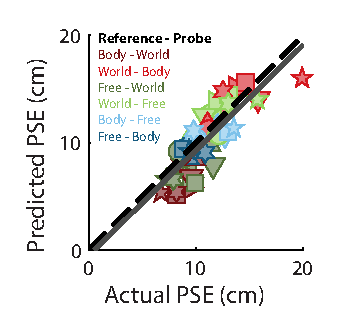
\includegraphics[width=0.5\textwidth]{src/paper4/p4_figure6.pdf}

    \caption{Predicted versus actual PSEs for Clemens \protect\citeyear{clemens2015a} using parameter $\alpha_{50}$ from the present paper. A data point (symbol) is shown for each participant (symbol shape) and condition (symbol color) pair, following the same color scheme as in \protect\figref{p3:fig2}: Body-world comparison; body reference, dark red; world reference, light red. World-free comparison; world reference, light green; free reference, dark green. Body-free comparison; body reference, dark blue; free reference, light blue.}
    \label{p4:fig6}
\end{figure}

In our previous experiment we compared body-fixed to world-fixed fixations at near (50 \si{\centi\metre}) distances only \cite{clemens2015a}. We compared the parameter, $\alpha$, found in that paper with the independently obtained parameter for the near condition, $\alpha_{50}$, from the present study. \figref{p4:fig6} shows how well our $\alpha_{50}$ parameter explains the data in our previous paper, the positive correlation between the actual PSEs and those predicted using the model in this paper ($\rho = 0.60$, $p = 0.06$) adds confidence to the parameter values presented here. The average difference between the values found here and those reported previously (see \tabref{p4:tab2}) is 12 \textpm 8 percent-points, indicating a variation of about 12\% on the contribution of the vestibular system versus that of the visual system between the present and our previous paper. While the variation might seem high, keep in mind that the two parameter values presented in this study are fitted on only four conditions, which do not overlap with the two conditions used to fit  parameter previously.

% Relation to the VOR
After showing that our present results in the nearby fixation condition are similar to those we found earlier, we go on and investigate to what extent the LVOR plays a role in the effects of eye movements on self-motion perception. Because the function of the LVOR is to keep the eyes stable in the world during linear translation, it also needs to scale with fixation depth \cite{paige1989, busettini1994,paige1998}. It is therefore possible that both the LVOR and self-motion perception have the same underlying same signal. Because of the visual fixation point, visual following mechanisms may even augment the LVOR compensation. If the oculomotor signal generated by the LVOR is the same signal that is used for self-motion perception, one would expect that the LVOR compensation at 50 and 200cm closely relate to the corresponding oculomotor weights in the present study (see \figref{p4:fig5} and \tabref{p4:tab2}). We derived the LVOR gains for 50 and 200 \si{\centi\metre} from Paige et al. \citeyear{1989} and computed their expected distance ratio, $d_{200} / d_{50}$. This ratio, 1.87, did not match either the ratio of the 6 participants who did not show any sign of scaling ($\frac{d_{200}}{d_{50}} = 1.07 \pm 0.16$) nor of the 2 participants that did show scaling ($\frac{d_{200}}{d_{50}} = 3.06 \pm 0.27$).

While we have shown that conscious perception of self-motion is influenced by eye movement, the same might not hold for actions based on self-motion. At the level of the vestibular system, it is known that perception of self-motion is influenced by the semicircular canals while the LVOR is not \cite{merfeld2005}, suggesting a more direct relation between the otolith signal and the LVOR. While it is unlikely that eye movements are used to drive the VOR because that would defeat the purpose of the eye movements themselves, we hypothesize that eye movements are also not used in other cases where latency is an important factor.


\subsection{Alternative explanations}

In addition to the absence of scaling, is is possible that eye movement information is integrated in a statistically optimal fashion, that is taking the noise in the vestibular and oculomotor signals into account. While the vestibular signal and thus noise is constant for a given translation distance, the noise in the oculomotor estimate might depend on both the magnitude of the eye movement (i.e. signal dependent noise) as well as on the  fixation depth.

 If signal dependent noise would play a role, we would expect the large eye movements in the near world stationary fixation condition to be noisier than the small eye movement in the far world stationary condition. This would cause the nearby oculomotor estimate to be weighted less than than the far away one and would reduce the magnitude of our effect and, if the difference in noise levels is large enough, could even invert it. Because signal dependent noise would  weaken the observed effect, we discard it as a possible alternative.
 
 In addition to signal dependent noise, the noise levels in the oculomotor estimate could also depend on fixation depth. The retinal displacement of a world stationary fixation point decreases with fixation depth, making it less informative about the amount of self-motion. The noise level in the oculomotor estimate would therefore be higher for far away compared to nearby fixation points. For world stationary targets, this would predict an underestimation of self-motion while fixating far away compared to nearby, which is in line with our observations. However, it also predicts a similar effect for body stationary targets. As no such effects between the near and far body stationary fixation targets have been observed, we consider it an unlikely alternative explanation.

Could the lack of scaling be explained by how participants perceive the far fixation point? Because the difference between body- and world-fixed fixation points is reduced at far fixation distances, the lack of scaling could - in theory - be explained by participants incorrectly perceiving both the body- and world-fixed far fixation points as being body-fixed. We consider this an unlikely explanation, because the target displacement associated with a world-fixed target was between 0.3 and 8.5 degrees in our experiment, which is easily perceivable especially given that the target was foveated. This adds confidence to our claim that eye movements indeed influence self-motion perception, but with moderate to no scaling for fixation depth.

\subsection{Conclusion}
% Conclusion
In summary, fixation depth is not properly taken into account, suggesting that a relatively raw eye movement signal is used in self-motion perception. While efference copies of the eye movement signals or proprioceptive feedback could be directly responsible for the perceived self-motion, it cannot be ruled out that the signals that drive the eye movements are not causing the reported effects instead.


% Talk about whether perception and action employ different mechanisms?
% Check work by Merfeld
%
% Vestibular perception and action employ qualitatively different mechanisms I and II
% Merfeld, Park, Gianna-Pulin, Black, Wood, 2005
%

% -- %

% Self-motion perception; disambiguation
% Rotation perception; do not expect fixation distance to play a role

% Link to path reception during rotation, influence of instructions, depth range, and dot density:
% Li Li, William H. Warren Jr. doi:10.1016/j.visres/2004.03.008

% Experimental Brain Research doi:10.1007/s00221-009-1828-z 123
% Eye eccentricity modifies the perception of whole-body rotation
% Gaelle Quarck, Lena Lhuisset, Olivier Etart, Pierre Denise